% !TEX program = xelatex
\documentclass[aspectratio=169,11pt]{beamer}

% --- Theme and Colors ---
\usetheme{Madrid}
\definecolor{ProfBlue}{RGB}{0,60,113}
\definecolor{LightBlue}{RGB}{220,235,252}
\definecolor{AccentBlue}{RGB}{30,100,180}
\definecolor{DarkGray}{RGB}{60,60,60}
\definecolor{TakeawayGreen}{RGB}{230,245,230}
\definecolor{TakeawayBorder}{RGB}{40,120,40}

\setbeamercolor{structure}{fg=ProfBlue}
\setbeamercolor{palette primary}{bg=ProfBlue,fg=white}
\setbeamercolor{palette secondary}{bg=AccentBlue,fg=white}
\setbeamercolor{palette tertiary}{bg=ProfBlue!80!black,fg=white}
\setbeamercolor{frametitle}{bg=ProfBlue,fg=white}
\setbeamercolor{title}{fg=white,bg=ProfBlue}
\setbeamercolor{block title}{bg=ProfBlue,fg=white}
\setbeamercolor{block body}{bg=LightBlue,fg=DarkGray}
\setbeamercolor{item}{fg=ProfBlue}

% --- Fonts ---
\usepackage{fontspec}
\setmainfont{Georgia}
\setsansfont{Georgia}

% --- Packages ---
\usepackage{booktabs}
\usepackage{graphicx}
\usepackage{amsmath}
\usepackage{tikz}
\usetikzlibrary{arrows.meta,positioning,shapes.geometric}
\usepackage{appendixnumberbeamer}

% --- Takeaway box ---
\newcommand{\takeaway}[1]{%
  \begin{tikzpicture}
    \node[fill=TakeawayGreen, draw=TakeawayBorder, rounded corners=4pt,
          inner sep=8pt, text width=0.92\textwidth, align=left] {%
      \textbf{Takeaway:} #1};
  \end{tikzpicture}%
}

% --- Number highlight ---
\newcommand{\hl}[1]{\textbf{\textcolor{ProfBlue}{#1}}}

% --- Navigation symbols off ---
\setbeamertemplate{navigation symbols}{}

% --- Slide numbers ---
\setbeamertemplate{footline}{%
  \hfill\insertframenumber/\inserttotalframenumber\hspace*{6pt}\vspace*{4pt}%
}

% --- Title info ---
\title[Unequal Equalization]{An Unequal Equalization}
\subtitle{Understanding the Response of Rates of Profit\\during the First Age of Globalization (1870--1913)}
\author{Kabeer Bora}
\date{}

% ============================================================
\begin{document}

% ------ SLIDE 1: Title ------
{
\setbeamertemplate{footline}{}
\begin{frame}[plain]
  \titlepage
\end{frame}
}

% ------ SLIDE 2: Motivation & Research Question ------
\begin{frame}{Motivation}
  \begin{itemize}
    \item The period \hl{1870--1913} is the \emph{First Age of Globalization} (O'Rourke \& Williamson, 2002)
    \item Unprecedented integration of commodity, capital, and labor markets
    \item Classical/Marxian political economy: foreign trade as a \emph{counteracting influence} to the tendency of the rate of profit to fall
    \item Yet no systematic empirical test of this mechanism exists
  \end{itemize}

  \vspace{0.5cm}
  \begin{block}{Research Question}
    Did trade openness raise national rates of profit during the First Age of Globalization, and if so, through which channel?
  \end{block}
\end{frame}

% ------ SLIDE 3: Theoretical Framework ------
\begin{frame}{Theoretical Framework}
  \textbf{Marx's Law of the Tendency of the Rate of Profit to Fall}
  \begin{itemize}
    \item Rising organic composition of capital $\Rightarrow$ downward pressure on $r = S / K$
    \item \emph{Counteracting influences} can offset or reverse this tendency
  \end{itemize}

  \vspace{0.3cm}
  \textbf{Foreign Trade as Counteracting Influence}
  \begin{itemize}
    \item \textbf{Export channel (surplus realization):} access to foreign markets allows realization of surplus value that cannot be absorbed domestically
    \item \textbf{Import channel (cheapening):} cheaper imported inputs reduce the value of constant and variable capital
  \end{itemize}

  \vspace{0.3cm}
  \takeaway{Trade openness should raise the rate of profit, primarily through the export channel --- surplus realization on global markets.}
\end{frame}

% ------ SLIDE 4: Data ------
\begin{frame}{Data: Seven Core Economies}
  \begin{columns}[T]
    \begin{column}{0.48\textwidth}
      \textbf{Countries}
      \begin{itemize}
        \item UK, USA, Germany, France
        \item Netherlands, Sweden, Spain
        \item Together: \hl{$\sim$63\%} of global trade
      \end{itemize}
      \vspace{0.3cm}
      \textbf{Panel structure}
      \begin{itemize}
        \item Balanced panel: \hl{308 obs} (7 $\times$ 44 years)
        \item Annual, 1870--1913
      \end{itemize}
    \end{column}
    \begin{column}{0.48\textwidth}
      \textbf{Key variables}
      \begin{itemize}
        \item \textbf{Net Rate of Profit} $r = \text{NOS}/K_{\text{net}}$
        \item Net productive capital stock (excl.\ residential dwellings, adjusted for depreciation)
        \item Mean $r$ = \hl{0.199}, SD = 0.113
      \end{itemize}
      \vspace{0.3cm}
      \textbf{Trade Openness}
      \begin{itemize}
        \item $(X+M)/\text{GDP}$
        \item Mean = \hl{0.441}
      \end{itemize}
    \end{column}
  \end{columns}
\end{frame}

% ------ SLIDE 5: Figure — Rate of Profit ------
\begin{frame}{Rate of Profit Trajectories, 1870--1913}
  \begin{center}
    \includegraphics[width=0.82\textwidth]{images_plots/all_rops.png}
  \end{center}
\end{frame}

% ------ SLIDE 6: Figure — Trade Openness ------
\begin{frame}{Trade Openness, 1870--1913}
  \begin{center}
    \includegraphics[width=0.82\textwidth]{images_plots/trade_openness_all_countries.png}
  \end{center}
\end{frame}

% ------ SLIDE 7: Empirical Strategy Overview ------
\begin{frame}{Empirical Strategy}
  \textbf{Baseline specification (TWFE):}
  \[
    r_{it} = \alpha_i + \gamma_t + \beta \cdot \text{Openness}_{it} + \mathbf{X}_{it}'\boldsymbol{\delta} + \varepsilon_{it}
  \]

  \begin{itemize}
    \item Country and year fixed effects absorb time-invariant heterogeneity and common shocks
    \item Controls: population growth, agricultural employment share, capital deepening
    \item \textbf{Problem:} endogeneity --- trade and profits jointly determined
  \end{itemize}

  \vspace{0.3cm}
  \textbf{Solution: Two-Stage Least Squares with two independent instruments}
  \begin{enumerate}
    \item \textbf{Climate instrument:} temperature uncertainty in partner countries $\times$ maritime distance $\times$ colonial ties (PPML gravity)
    \item \textbf{Pascali (2017) instrument:} sail-to-steam transition travel times
  \end{enumerate}

  \vspace{0.2cm}
  \takeaway{Two instruments exploit entirely different variation: demand-side annual weather shocks vs.\ supply-side secular technological change.}
\end{frame}

% ------ SLIDE 8: IV — Climate Instrument with DAG ------
\begin{frame}{IV Strategy: Climate Uncertainty Instrument}
  \begin{center}
    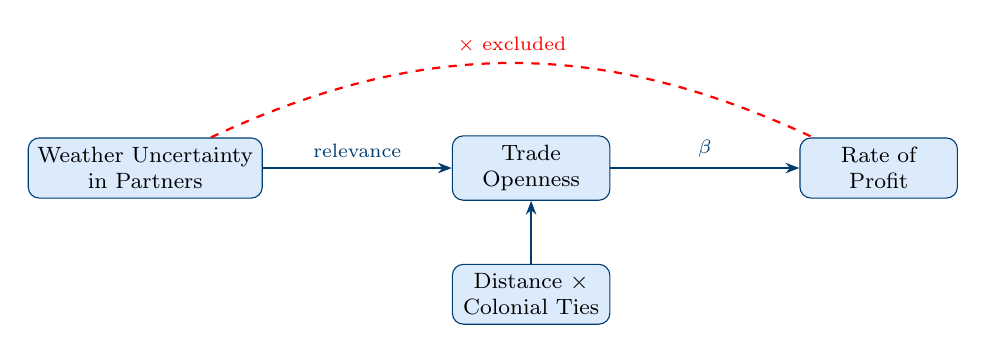
\begin{tikzpicture}[
      node distance=0.8cm and 2.4cm,
      every node/.style={font=\footnotesize},
      box/.style={rectangle, draw=ProfBlue, fill=LightBlue, rounded corners,
                  minimum height=0.7cm, minimum width=2cm, align=center},
      arr/.style={-{Stealth[length=5pt]}, thick, ProfBlue}
    ]
      \node[box] (Z) {Weather Uncertainty\\in Partners};
      \node[box, right=of Z] (T) {Trade\\Openness};
      \node[box, right=of T] (Y) {Rate of\\Profit};
      \node[box, below=of T] (G) {Distance $\times$\\Colonial Ties};

      \draw[arr] (Z) -- node[above, font=\scriptsize]{relevance} (T);
      \draw[arr] (T) -- node[above, font=\scriptsize]{$\beta$} (Y);
      \draw[arr] (G) -- (T);
      \draw[thick, red, dashed] (Z) to[bend left=25] node[above, font=\scriptsize, red]{$\times$ excluded} (Y);
    \end{tikzpicture}
  \end{center}

  \vspace{0.2cm}
  \begin{columns}[T]
    \begin{column}{0.48\textwidth}
      \textbf{Construction}
      \begin{itemize}
        \item Partner temperature uncertainty $\times$ maritime distance $\times$ colonial ties
        \item PPML gravity $\to$ predicted openness
        \item First-stage F \hl{$>$ 50}
      \end{itemize}
    \end{column}
    \begin{column}{0.48\textwidth}
      \textbf{Exclusion restriction}
      \begin{itemize}
        \item Weather shocks in distant partners affect profits \emph{only through trade}
        \item Domestic climate controlled directly in 2nd stage
      \end{itemize}
    \end{column}
  \end{columns}
\end{frame}

% ------ SLIDE 9: IV — Pascali Instrument ------
\begin{frame}{IV Strategy: Pascali (2017) Instrument}
  \begin{itemize}
    \item Exploits the \textbf{sail-to-steam transition} in maritime shipping
    \item Differential reduction in bilateral travel times depending on geography (winds, currents, coaling stations)
    \item Generates exogenous, time-varying predicted trade shares
  \end{itemize}

  \vspace{0.3cm}
  \begin{columns}[T]
    \begin{column}{0.48\textwidth}
      \begin{block}{Identifying Variation}
        Supply-side, secular technological shock --- independent of annual demand conditions
      \end{block}
    \end{column}
    \begin{column}{0.48\textwidth}
      \begin{block}{First-Stage Strength}
        F-statistic \hl{$>$ 10}
      \end{block}
    \end{column}
  \end{columns}

  \vspace{0.3cm}
  \takeaway{Two instruments are complementary: climate captures short-run demand shocks; Pascali captures long-run supply-side integration.}
\end{frame}

% ------ SLIDE 10: TWFE Results ------
\begin{frame}{TWFE Results (Suggestive)}
  \begin{center}
    \begin{tabular}{lcc}
      \toprule
      & Coefficient on Openness & Wild-cluster bootstrap $p$ \\
      \midrule
      Across 6 specifications & \hl{0.032--0.039} & 0.21--0.41 \\
      \bottomrule
    \end{tabular}
  \end{center}

  \vspace{0.4cm}
  \begin{itemize}
    \item Sign is consistently positive
    \item But inference is fragile: wild-cluster bootstrap $p$-values \hl{0.21--0.41} with only $G=7$ clusters
    \item Does \textbf{not} survive conventional significance thresholds
  \end{itemize}

  \vspace{0.3cm}
  \takeaway{TWFE provides suggestive evidence of a positive relationship. Causal identification requires IV.}
\end{frame}

% ------ SLIDE 11: IV Main Results ------
\begin{frame}{IV Results: Main Finding}
  \begin{center}
    \begin{tabular}{lcc}
      \toprule
      Instrument & Bare & Full Controls \\
      \midrule
      Climate        & \hl{0.325}*** (0.062) & \hl{0.317}*** (0.064) \\
      Pascali        & \hl{0.311}*** (0.072) & \hl{0.296}** \phantom{*}(0.094) \\
      \bottomrule
    \end{tabular}
  \end{center}

  \vspace{0.3cm}
  \begin{itemize}
    \item A \hl{1 pp} increase in trade openness $\rightarrow$ \hl{0.30--0.33 pp} increase in the net rate of profit
    \item At the mean $r \approx 20\%$, this represents a \hl{1.5--1.7\%} relative increase
    \item Estimates are \textbf{remarkably stable} across instruments and specifications
  \end{itemize}

  \vspace{0.3cm}
  \takeaway{Both instruments yield consistent, large, positive effects of trade openness on the rate of profit.}
\end{frame}

% ------ SLIDE 12: IV Robustness ------
\begin{frame}{IV Robustness}
  \textbf{Overidentification}
  \begin{itemize}
    \item Sargan--Hansen $J$: \hl{2.84} ($p=0.092$) bare; \hl{3.34} ($p=0.067$) full controls
    \item Does not reject at 5\% --- instruments are mutually consistent
  \end{itemize}

  \vspace{0.3cm}
  \textbf{Leave-One-Out (LOO) Analysis}
  \begin{itemize}
    \item Drop each country in turn $\Rightarrow$ 7 subsamples
    \item \textbf{All 7} estimates are positive
    \item Range: \hl{0.227--0.429}
    \item No single country drives the result
  \end{itemize}

  \vspace{0.3cm}
  \takeaway{Results are robust to overidentification testing and are not driven by any single country.}
\end{frame}

% ------ SLIDE 13: Export vs Import Channel ------
\begin{frame}{Export vs.\ Import Channel Decomposition}
  \begin{center}
    \begin{tabular}{lcc}
      \toprule
      Channel & IV Coefficient & First-stage $F$ \\
      \midrule
      Export / GDP (instrumented)  & \hl{0.302***--0.350**} & $>10$ \\
      Import / GDP (instrumented)  & 0.157--0.191          & $<10$ (weak) \\
      \bottomrule
    \end{tabular}
  \end{center}

  \vspace{0.4cm}
  \begin{itemize}
    \item The \textbf{export channel} is statistically significant and economically large
    \item The import channel is insignificant, and the instrument is weak for imports
    \item Consistent with the Marxian mechanism: \emph{surplus realization on global markets}
  \end{itemize}

  \vspace{0.3cm}
  \takeaway{Exports, not imports, drive the trade--profit nexus. This supports the surplus realization interpretation.}
\end{frame}

% ------ SLIDE 14: Convergence ------
\begin{frame}{Convergence of Rates of Profit}
  \textbf{Beta-convergence}
  \begin{itemize}
    \item Coefficient: $\hat{\beta} =$ \hl{0.019--0.028}
    \item Half-life: \hl{25--36 years}
    \item Countries with higher initial $r$ experience slower profit growth $\Rightarrow$ convergence
  \end{itemize}

  \vspace{0.3cm}
  \textbf{Sigma-convergence}
  \begin{itemize}
    \item Cross-country dispersion of $r$ is \textbf{non-monotone}
    \item Peaks $\sim$1880, trough $\sim$1885, then widens again
    \item No sustained reduction in dispersion over the full period
  \end{itemize}

  \vspace{0.3cm}
  \takeaway{Beta-convergence confirms a Marxian ``tendency'' toward equalization, but sigma-convergence shows it was \emph{unequal} and incomplete.}
\end{frame}

% ------ SLIDE 15: Figure — Sigma Convergence ------
\begin{frame}{Sigma-Convergence: Cross-Country Dispersion of $r$}
  \begin{center}
    \includegraphics[width=0.82\textwidth]{images_plots/sigma_convergence_plot_1.png}
  \end{center}
\end{frame}

% ------ SLIDE 16: Conclusion ------
\begin{frame}{Conclusion}
  \textbf{Summary of findings}
  \begin{enumerate}
    \item Trade openness raised national rates of profit during 1870--1913
    \item The effect is large: \hl{0.30--0.33 pp} per 1 pp increase in openness
    \item The \textbf{export channel} (surplus realization) drives the result
    \item Rates of profit show beta-convergence but incomplete sigma-convergence --- an ``unequal equalization''
  \end{enumerate}

  \vspace{0.3cm}
  \textbf{Contributions}
  \begin{itemize}
    \item First systematic IV estimates of trade--profit nexus in the 19th century
    \item Novel climate-based instrument for historical trade
    \item Empirical support for Marx's foreign-trade counteracting influence
    \item Nuances the equalization narrative: convergence in tendency, not in outcome
  \end{itemize}
\end{frame}

% ------ SLIDE 17: Thank You ------
{
\setbeamertemplate{footline}{}
\begin{frame}[plain]
  \begin{center}
    \vspace{2cm}
    {\Large\textbf{\textcolor{ProfBlue}{Thank you}}}

    \vspace{1cm}
    {\large Questions and comments welcome.}
  \end{center}
\end{frame}
}

\end{document}
